%----------------------------------------
% Write your notes here
%----------------------------------------

\section{Major Topics Covered}
\begin{itemize}
  \item Classification as a Regression Problem
  \item Introducing Logistic Regression
  \item Interpreting Logistic Regression
  \item Exploring Vowpal Wabbit
  \item Introduction to Networks
\end{itemize}


\section{Classification as a Regression Problem}

Why do we bother with Logistic Regression, when a simple regression model could be used for our classification problem? Linear regression returns a real number, which we can then convert to a class.

We can have a dependent variable 'y' and a set of independent features 
\begin{equation}
  x \in R ^{d}
\end{equation}
As seen in Linear Regression, we fit a model :
\begin{equation}
  \hat{y} = w.x
\end{equation}
where w is the vector of weights.

Analyzing the performance of this model using the previously introduced Least Square approach, we begin to see a problem. Consider fitting a regression line to this plot. Our 'y' will definitely be a real number, but we want it to be a class.

\begin{figure}[ht]
  \begin{center}
    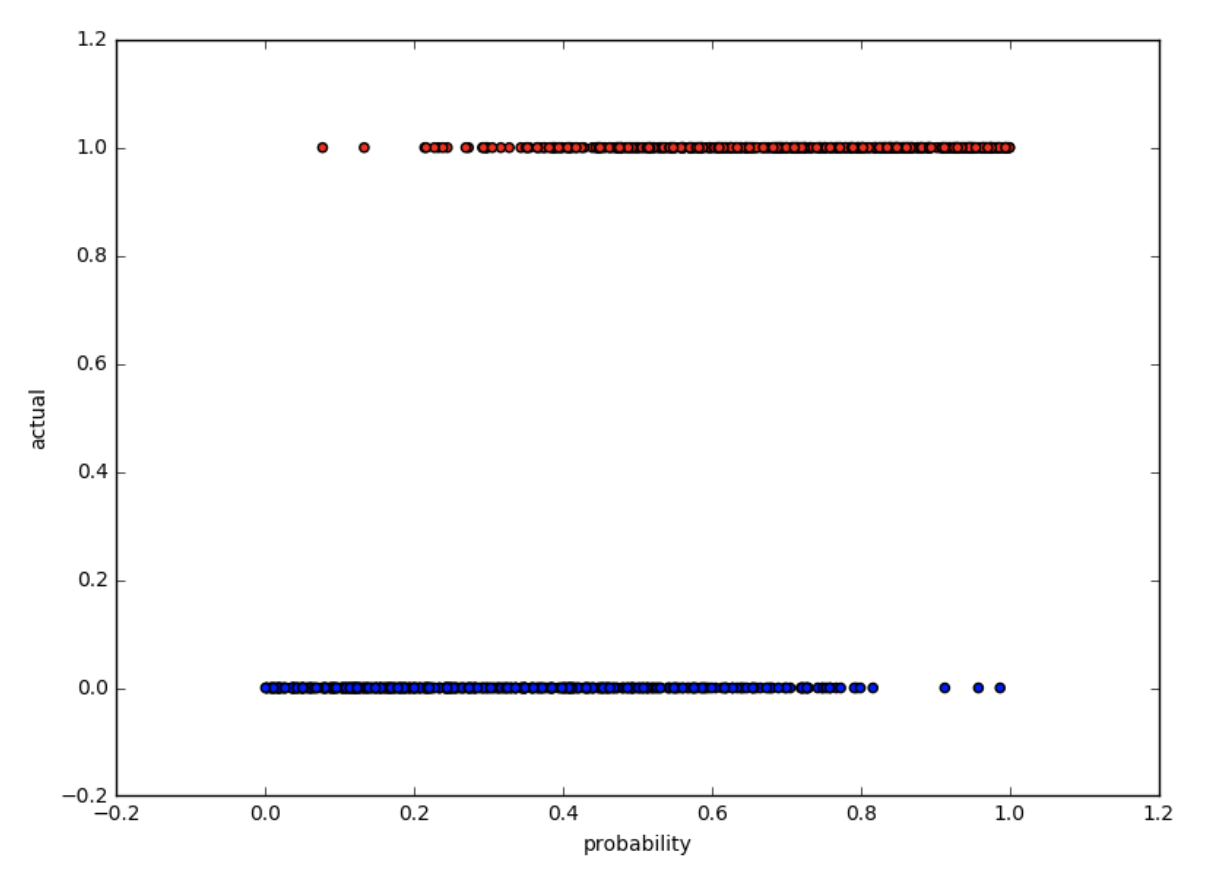
\includegraphics[width=0.5\textwidth]{figures/fig-1.png}
    \caption{}
    \label{fig:example_figure}
  \end{center}
\end{figure}

Using Least Squares method to analyze our model performance on fitting a straight line, as always: 
\begin{equation}
  LSE = 1/n \sum_{i}(\hat{y _{i}} - y _{i})^2
\end{equation}

Error rates aren't representative of actual errors, since the points that were classified correctly will also give a non-zero error.

But fret not, we can fix this with a hack - a very simple case of clipped or piecewise linear regression. This way, all predicted values above 1 will be set to 1, and all predicted values less than 0 will be set to 0.

We'll see that logistic regression is a more eloquent way of handling this issue.

\section{Introducing Logistic Regression}

When we've restricted our response variable to $ y \in {0,1}$, 
logistic regression provides a solution by fitting our model to the log odds rather than the class of y.

The resulting fit equation is given by :
\begin{equation}
  ln(\frac{p}{1-p}) = w.x
\end{equation}

Loss is calculated as : 
\begin{equation}
  L=\prod_{i=i} p_i^{y_i}(1-p_i)^{1-y_i}
\end{equation}

\begin{figure}[ht]
  \begin{center}
    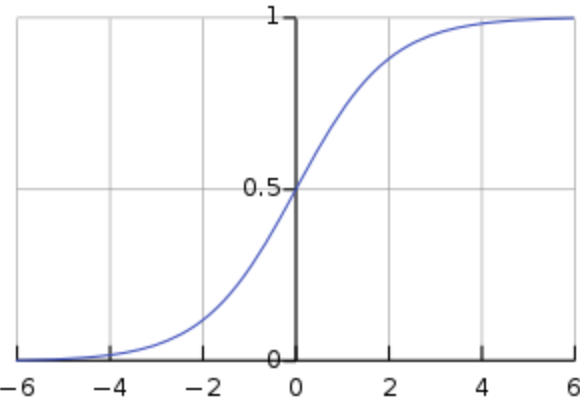
\includegraphics[width=0.5\textwidth]{figures/fig-2.png}
    \caption{}
    \label{fig:example_figure2}
  \end{center}
\end{figure}

The resulting sigmoid eliminates the loss problem that we saw in the previous section. 

\section{Interpreting Logistic Regression}

We considered the Titanic dataset to predict whether a person survived or drowned, based on Gender first. 
\begin{figure}[ht]
  \begin{center}
    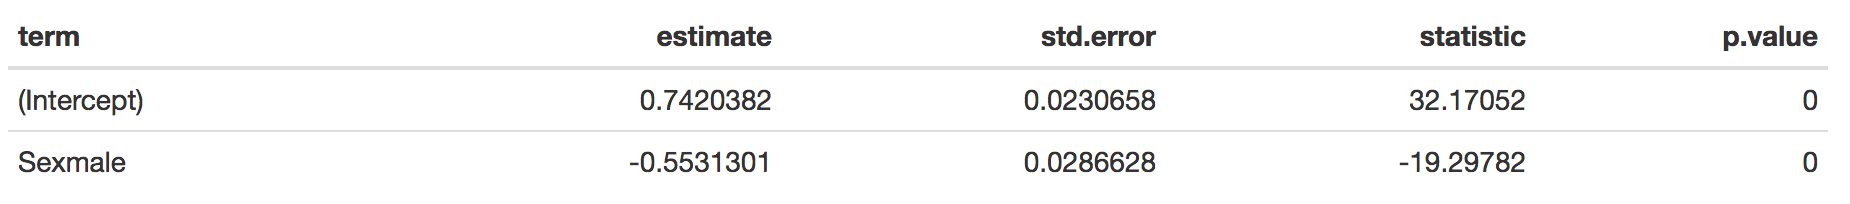
\includegraphics[width=0.5\textwidth]{figures/fig-3.png}
    \caption{}
    \label{fig:example_figure3}
  \end{center}
\end{figure}

Let us now interpret this table. The 'sexmale' estimate tells us the change in log odds of male survival per unit increase. The 'intercept' refers to the odds of a zero year old male surviving. We use the following equation to interpret the values returned by summary :
\begin{equation}
  p(y=1|x,w) = 1/(1+e(-wx))
\end{equation}

So, for instance, we want to compute the survival odds of a person given a host of variables (with respective coefficients obtained from the summary) about them, here's the formula :
\begin{equation}
  survival-prob = 1/(1+exp(-(coef_{1}*val_{1} +coef_{2}*val_{2} + coef_{3}*val_{3} + ...)))
\end{equation}

where $ coef_{i}$ was obtained from the summary, and $val_{i}$ are values that the feature takes.

*The discussion digressed to how the error bar can be obtained for regression model - solution is to use different samples, and generate fits for them. Get a 95\% confidence interval and use convex hull.



\section{Vowpal Wabbit}

Here's a few takeaways from our tutorial on Vowpal Wabbits :
\begin{itemize}
  \item Has some advantages over traditional packages - such as scalability and feature pairing.
  \item Uses progressive validation instead of cross validation - loss reduces over iterations.
  \item Accepts input in a very flexible and convenient format (esp for our news example) - just enter the list of words occuring in each row.
  \item Learning Algorithm is very fast as demonstrated in class.
\end{itemize}

\section{Introduction to Networks}
An assumption so far has been that the individual observations are Independent. With Networks we assume a relational dependence, i.e the observations are interconnected at some abstract level. 

Let us go through the history of Networks :
\begin{enumerate}
  \item An early paper analyzing social networks, by Granovetter titled "Strength of Weak Ties" argues that the "degree of overlap of friendship networks" (i.e mutual friends) is proportional to the strength of their friendship. 
  
  We also saw the distribution of social networks can be defined as clusters of strong ties, that are connected with weak ties. The paper stresses on the power these weak ties between groups can wield.
  
  This also ties to a pattern often observed in academia, and in general - of "cumulative advantage" , i.e the rich getting richer. An example we observed was that of the number of citations per paper. A tiny minority of papers get cited a lot, whereas the vast majority have very few citations.
  
  \item Erdos and Renyi worked on Random Graph Theory - probabilistic models. Each edge has a probability of existing - how high does the probability have to be for a set of users to be connected.
  
  \item Small World Networks were introduced in the 90s, after Watts and Stogartz observed that many real world networks had small average shortest paths between any two random nodes (as observed in the ER pure Random graphs) but a higher clustering coefficient. 
  
  This high clustering coefficient results in a bunch of high degree nodes called "hubs" that result in shorter average path lengths that are observed in real life scenarios (eg the "6 degrees of separation").
    
  \item In the modern times, we have a lot of social network data at our disposal. We observed a visualization made using blog data that showed the polarization between Republican and Democrat supporters.
  
\end{enumerate}

We discussed the various types of networks that are in use today - for instance "Social Media" - sites like Facebook where there is an explicit definition of the relationship between 2 users as 'friends'/'connections'.
Then there's Geographical networks like Google Maps.

Representing networks can be done with varying degrees of Abstraction - for instance undirected networks indicate only a link between two nodes whereas directed networks give a direction/causation info.

We discussed different ways of visualizing networks - for instance in Facebook networks we could perhaps restrict the visualization to only the active connections, or perhaps to reciprocating connections to gather better insight.
We saw an example of such 'encoding', where the emails sent within an organization were used to deduce reporting relationships (darker lines) and email communication (other lines) between the various senders and receivers.

There are a few ways of Representing Networks :

\begin{enumerate}
  \item Edge List : 
  \begin{itemize}
    \item Simply stores a list of the connected edges in the graph/network.
    \item Simple for storage
    \item Complex computations, finding all points adjacent to a node requires O(e) where 'e' is the number of edges.
  \end{itemize}
  \item Adjacency Matrix : 
  \begin{itemize}
    \item A matrix that stores a 0 or 1 indication presence of edge between all edge (n1,n2) combinations.
    \item Higher space complexity \begin{equation}O(n^{2})\end{equation}
    \item Lower computational complexity - for instance finding all neighbours of given node takes \begin{equation}O(n)\end{equation}
    \item Finding whether an edge exists is super fast - \begin{equation}O(1)\end{equation}
  \end{itemize}
  \item Adjacency List : 
  \begin{itemize}
    \item An array of all nodes, where each element points to a linked list of adjacent nodes.
    \item Not the best structure for checking if an edge exists, will take \begin{equation}O(avg-degree)\end{equation}
    \item However good for getting all the neighbours, hence traversal.
  \end{itemize}
    
\end{enumerate}
Describing our Network can use many parameters, for instance degree distributions - say there are lots of 3-4 way intersections. We've discussed some others, like the distance between two nodes (in history of networks), groups (tightly knit clusters).
\end{document}
